\documentclass{article}
\usepackage{tikz}
\usetikzlibrary{shapes.geometric, arrows}



\begin{document}

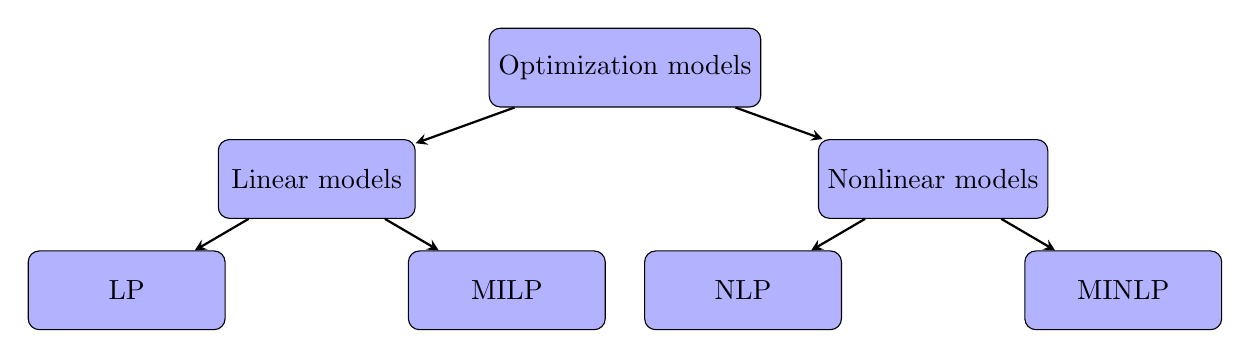
\begin{tikzpicture}[node distance=2cm and 2.5cm]
\tikzstyle{box} = [rectangle, rounded corners, minimum width=2.5cm, minimum height=1cm, text centered, draw=black, fill=blue!30]
\tikzstyle{arrow} = [thick,->,>=stealth]
% Nodes
\node (optimization) [box] {Optimization models};
\node (linear) [box, below left of=optimization, xshift=-2.5cm] {Linear models};
\node (nonlinear) [box, below right of=optimization, xshift=2.5cm] {Nonlinear models};
\node (lp) [box, below left of=linear, xshift=-1cm] {LP};
\node (milp) [box, below right of=linear, xshift=1cm] {MILP};
\node (nlp) [box, below left of=nonlinear, xshift=-1cm] {NLP};
\node (minlp) [box, below right of=nonlinear, xshift=1cm] {MINLP};

% Arrows
\draw [arrow] (optimization) -- (linear);
\draw [arrow] (optimization) -- (nonlinear);
\draw [arrow] (linear) -- (lp);
\draw [arrow] (linear) -- (milp);
\draw [arrow] (nonlinear) -- (nlp);
\draw [arrow] (nonlinear) -- (minlp);

\end{tikzpicture}

\end{document}
